\documentclass[crop]{standalone}

% convert to png with ``pdftoppm articubench_overview.pdf articubench_overview -png``

\usepackage{tikz}

\usetikzlibrary{arrows,shapes,calc,backgrounds,arrows.meta}
\usetikzlibrary{positioning}
\definecolor{celadon}{rgb}{0.67, 0.88, 0.69}
\definecolor{corn}{rgb}{0.98, 0.93, 0.36}
\definecolor{cottoncandy}{rgb}{1.0, 0.74, 0.85}
\definecolor{bluegray}{rgb}{0.4, 0.6, 0.8}
\definecolor{crimson}{rgb}{0.86, 0.08, 0.24}
\definecolor{forestgreen}{rgb}{0.13, 0.55, 0.13}
\definecolor{awesome}{rgb}{1.0, 0.13, 0.32}

\definecolor{kaminrot}{RGB}{165,30,55}
\definecolor{anthrazit}{RGB}{50,65,75}
\definecolor{gold}{RGB}{180,160,105}
\definecolor{blaugrau}{RGB}{0, 105, 170}
\definecolor{gelbbraun}{RGB}{210,150,0}
\definecolor{lilagrau}{RGB}{175,110,150}
\definecolor{grüngrau}{RGB}{130,185,160}
\definecolor{waldgrün}{RGB}{50,110,30}
\definecolor{apfelgrün}{RGB}{125,165,75}

\makeatletter
\newcommand{\gettikzxy}[3]{%
  \tikz@scan@one@point\pgfutil@firstofone#1\relax
  \edef#2{\the\pgf@x}%
  \edef#3{\the\pgf@y}%
}
\makeatother

\begin{document}

\tikzstyle{data}=[draw, fill=bluegray!60, text width=17em, text centered, minimum height=10em]
\tikzstyle{target}=[data, fill=forestgreen!20]
\tikzstyle{evaluation}=[data, fill=bluegray!20, text=awesome]
\tikzstyle{predictive} = [data, fill=corn!20, rounded corners]
\tikzstyle{vtl} = [data, fill=corn!60, rounded corners]

\begin{tikzpicture}[to/.style={->,ultra thick,shorten >=3pt,black}]

    % Data in articubench
    \node (target_semantic) [target]  {{\huge \bf target semantics}};
    \path (target_semantic.south)+(0.0, -14.24) node (target_acoustic) [target]  {{\huge \bf target acoustics}};
    \path (target_acoustic.east)+(10.0, 0.0) node (cp) [data] {{\huge \bf cp-trajectories}};
    \path (cp.east)+(8.0, 0.0) node (vtl) [vtl]  {{\huge \bf VocalTractLab}};
    \path (vtl.east)+(6.0, 0.0) node (audio) [data]  {{\huge \bf synthesized audio}};
    \path (audio.east)+(6.0, 0.0) node (acoustic) [data]  {{\huge \bf acoustic \\ representation}};
    \path (acoustic.east)+(5.0, 8.0) node (embedder) [predictive]  {{\huge \bf Embedder}};
    \path (embedder.west)+(-5.0, 8.0) node (semantic) [data]  {{\huge \bf semantic representation}};

    \draw[to,-{Latex[scale=2.0]}] (cp.east) to (vtl.west);
    \draw[to,-{Latex[scale=2.0]}] (vtl.east) to (audio.west);
    \draw[to,-{Latex[scale=2.0]}] (audio.east) to (acoustic.west);
    \draw[to,-{Latex[scale=2.0]}] (acoustic.east) to[bend right] (embedder.south);
    \draw[to,-{Latex[scale=2.0]}] (embedder.north) to[bend right] (semantic.east);


    % Tasks
    \draw[to,forestgreen,line width=4pt,-{Latex[scale=1.0]}] (target_semantic.south east) to node[midway, text centered]{{\huge \bf semantic only}}(cp.north);
    \draw[to,forestgreen,line width=4pt,-{Latex[scale=1.0]}] (target_acoustic.east) to node[midway, above=0.2cm, text centered]{{\huge \bf acoustic only}} (cp.west);
    \draw[to,forestgreen,line width=4pt,-{Latex[scale=1.0]}] (target_acoustic.north) -- (0.0, -8.0) to node[midway, above=-0.2cm, text centered]{{\huge \bf semantic-acoustic}} (cp.north west);
    \draw[to,forestgreen,line width=4pt,-{Latex[scale=1.0]}] (target_semantic.south) -- (0.0, -8.0) to (cp.north west);


    % Scores
    \path (cp.east)+(8.0, -8.0) node (vel_jerk) [evaluation]  {{\huge \bf Velocity loss\\Jerk loss}};
    \path (vtl.east)+(6.0, -4.0) node (ema) [evaluation]  {{\huge \bf EMA sensors}};
    \path (vtl.east)+(6.0, -8.0) node (ultra_sound) [evaluation]  {{\huge \bf midsagittal slice (ultra sound)}};
    \path (audio.east)+(6.0, -4.0) node (loudness) [evaluation]  {{\huge \bf loudness envelope}};
    \path (audio.east)+(6.0, -8.0) node (formants) [evaluation]  {{\huge \bf pitch; formants}};

    \draw[to,bluegray,-{Latex[scale=2.0]}] (cp.south east) to (vel_jerk.west);
    \draw[to,bluegray,-{Latex[scale=2.0]}] (vtl.south east) to (ema.west);
    \draw[to,bluegray,-{Latex[scale=2.0]}] (vtl.south east) to (ultra_sound.west);
    \draw[to,bluegray,-{Latex[scale=2.0]}] (audio.south east) to (loudness.west);
    \draw[to,bluegray,-{Latex[scale=2.0]}] (audio.south east) to (formants.west);
    \draw[dashed,awesome,line width=4pt] ($(target_semantic.east)+(0,0)$) -- node[midway,above=0.2cm, text centered]{{\huge \bf semantic RMSE ~loss; classification rank}} node[midway,black,below=0.2cm,text width=17em, text centered]{} ($(semantic.west)+(0, 0)$);
    \draw [dashed,awesome,line width=4pt] (acoustic.north)  -- +(0,+3.75) -- node[pos = 0.25, above = 0.2cm, text centered]{{\huge \bf acoustic RMSE ~loss}} node[midway,black,below left = 0.2cm and 1.4cm,text width=17em, text centered]{} ($(target_acoustic.north) + (1,4.)$) -- ($(target_acoustic.north) + (1, 0)$);
        
    

%     % embed external images
     \begin{scope}[on background layer]
    
    \node (vtl-figure) at ($(vtl.south)+(-2.1,3.2)$)
     {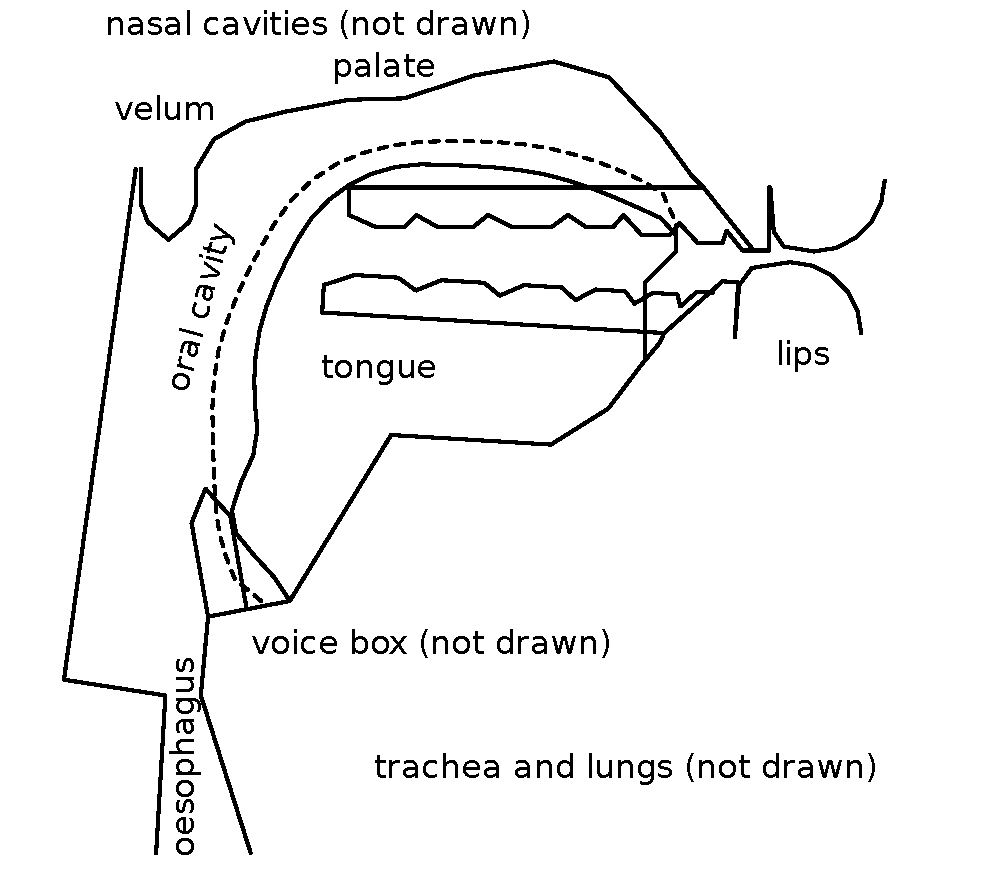
\includegraphics[width=1.\textwidth]{tract00000_no_frame.pdf}};
    
     \node (synthesized-wave) at ($(audio.north)+(-1.0, 1.2)$)
     {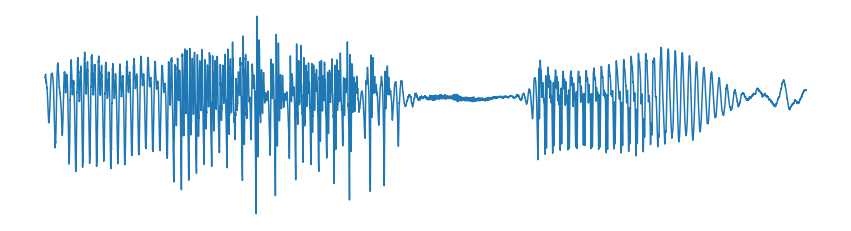
\includegraphics[width=.6\textwidth]{wav_no_frame.png}};
     
     \node (embedding) at ($(semantic.south)+(-8, -3)$)
     {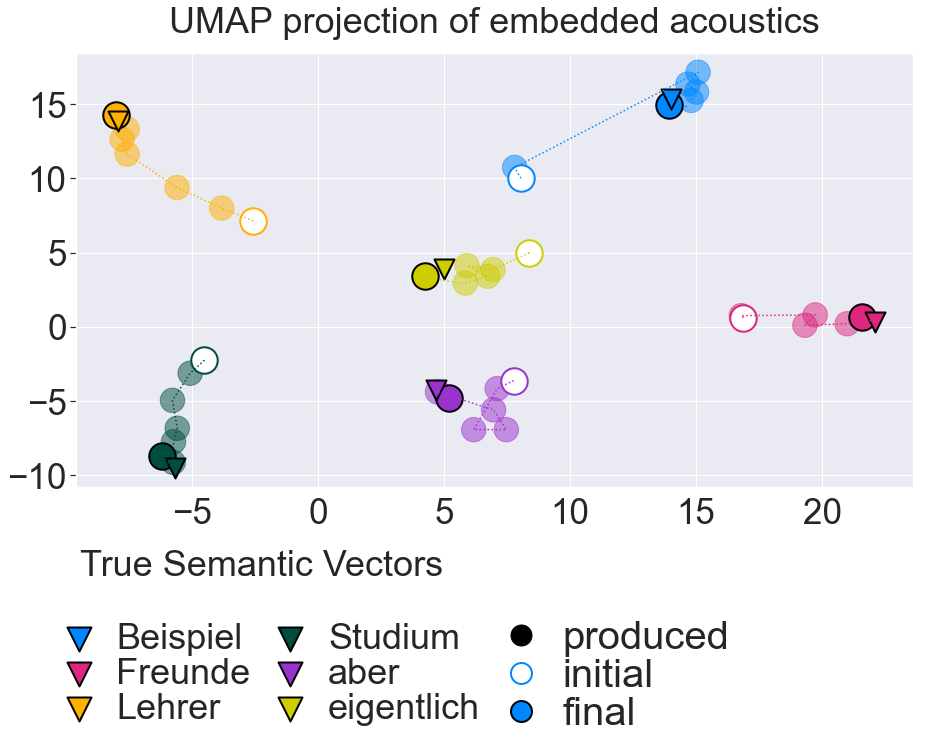
\includegraphics[width=0.9\textwidth]{umap_planned.png}};
     
     \node (melspec) at ($(target_acoustic.south)+(0, -2)$)
     {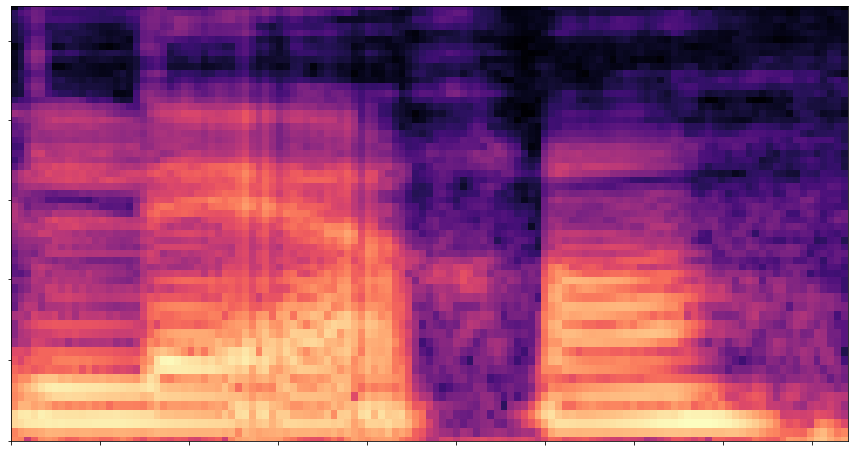
\includegraphics[width=.53\textwidth]{logmelspec.png}};
     
     \node (melspec) at ($(acoustic.north)+(4, 1.5)$)
     {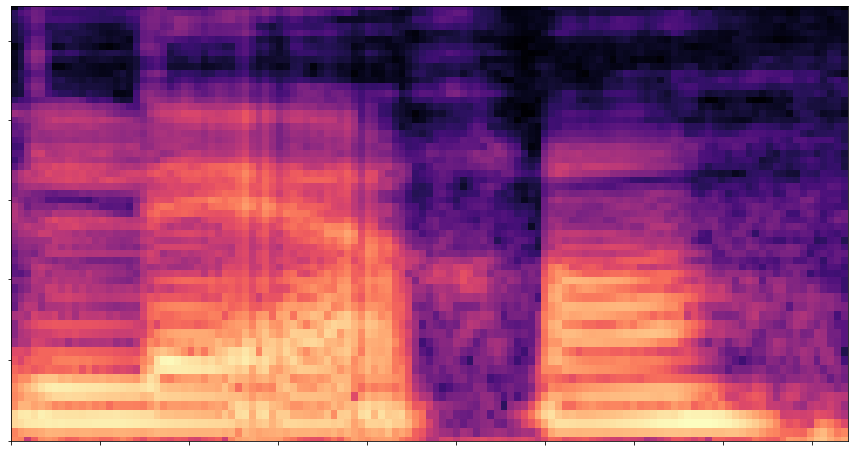
\includegraphics[width=.53\textwidth]{logmelspec.png}};
     
     \node (cps) at ($(cp.south)+(0, -2.0)$)
     {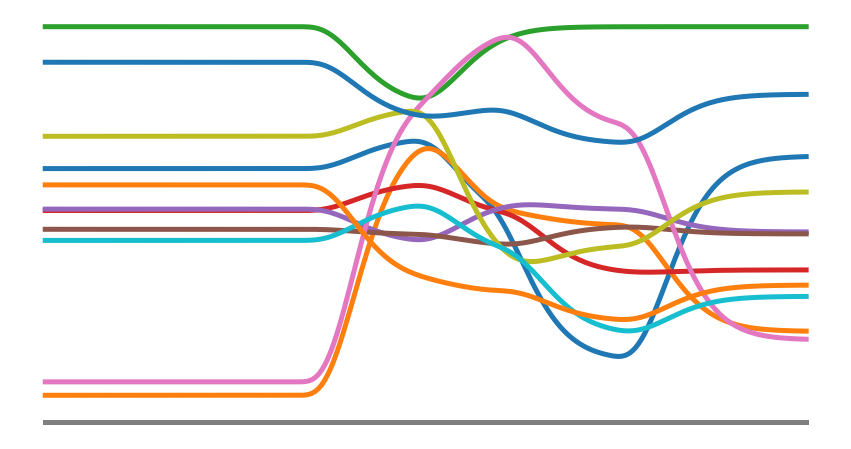
\includegraphics[width=.53\textwidth]{cps_no_frame.png}};
     
    \end{scope}
\end{tikzpicture}
%}
\end{document}
